\documentclass[final,3p,times,twocolumn,sort&compress]{elsarticle}
\usepackage{graphicx}
\usepackage{url}
\usepackage{subfig,natbib}
\usepackage{caption,multirow,float}
\usepackage{stfloats,graphicx,wrapfig}
\usepackage[all]{xy}
\usepackage[cmex10]{amsmath}
\usepackage{amssymb}
\usepackage{booktabs,mathrsfs,multirow}
\usepackage{color, colortbl}
\usepackage[table]{xcolor}
\definecolor{color1}{RGB}{0,0,0}
\definecolor{color2}{RGB}{64,64,64}
\definecolor{dkgreen}{rgb}{0,0.6,0}
\definecolor{gray}{rgb}{0.5,0.5,0.5}

\usepackage{multicol}
\usepackage{listings}
\lstset{language=Matlab}
\lstset{flexiblecolumns=true}
\usepackage{amssymb,epstopdf}
\usepackage[none]{hyphenat}
\usepackage[pagebackref=true,colorlinks=true]{hyperref}
\usepackage{balance}
 \biboptions{}
\journal{Applied soft computing}
\sloppy
\begin{document}

\begin{frontmatter}


\makeatletter
\title{PRE-PROCESSING TECHNIQUES}
\author[S1]{PRASHANTH G L}
\ead{guledalprashanth@gmail.com}
\author[S2]{CHARAN S G}
\ead{charansg333@gmail.com}

\cortext[cor1]{Corresponding author}
\address[S1]{1MS10EC083 Electronics and Comm, M S Ramaiah Institute of Technology}
\address[S2]{1MS10EC023 Electronics and Comm, M S Ramaiah Institute of Technology}

\begin{abstract}

Many complex problems arises in the Face Recognition Systems due to various reasons such as varying light, background,noise etc.These problems has to be first addressed  by applying some sort of processing to images before they are analysed in order to enhance  the reliability of  face recognition .Here the solution is provided to some of these problems through various pre-processing techniques.These include Scale Normalization, background removal,illumination invariance,template matching,skin color segmentation and 2D Normalized cross correlation.

\end{abstract}
\begin{keyword}
Face Recognition  \sep Scale normalization  \sep Background removal \sep Illuminations variations  \sep Template matching \sep Skin color segmentation \sep 2D Normalized Cross Correlation
\end{keyword}
\end{frontmatter}

\section{Introduction}
 \hspace{.11cm} Varying poses, expressions, troubling background, \\ various light interferences,noisy conditions, etc., makes \\ the recognition of the faces difficult. Using the proper preprocessing techniques we can make the faces invariant towards all the above effects.The uphill task lies in developing the optimised preprocessing techniques as it needs to suppress the information that is not relevant and to preserve the necessary features which helps us to identify the face and differentiate it from others.Next sections describe various processing steps to make the face recognition easy before the processing of images begin.
\section{Pre-Processing}
\subsection{Scale Normalization}
\hspace{1cm} The most important method of pre-processing is Scale normalisation \cite{One} . It is used when we use the Euclidean rules(ER) of testing.
If we are trying to match between two figures which are taken from different distances using Euclidean rule, we get an erroneous result. To overcome this error one has to get the pictures from the same distance, this method of converting variable scaled pictures to uniform scaled pictures is Scale normalisation.
 \begin{table}[htbp]
  \begin{center}
  \begin{tabular}{cc}
  \includegraphics[width=3.3cm,height=3.3cm]{Scale1} &  \includegraphics[width=3.3cm,height=3.3cm]{Scale2} \\
     \end{tabular}
Fig-1:- Figure depicting the facial image before and after scale normalisation
 \end{center}
 \end{table}

\textbf{Algorithm}

\begin{itemize}
  \item The skin segmentation is done to the image which has to be scaled.
  \item The boundaries of the skin segmented region are marked and are extracted out.
  \item The irregularities, discontinuities in the skin are also taken into consideration and is removed using the maximum feature technique.
\end{itemize}

\subsection{Background removal}
\hspace{1cm} To remove the redundant features in the figure we employ a technique called background removal. Here it is taken care that the pixels of background are nullified\cite{three} . This helps in good recognition if using the ER.\\
\begin{table}[htbp]
  \begin{center}
  \begin{tabular}{cc}
  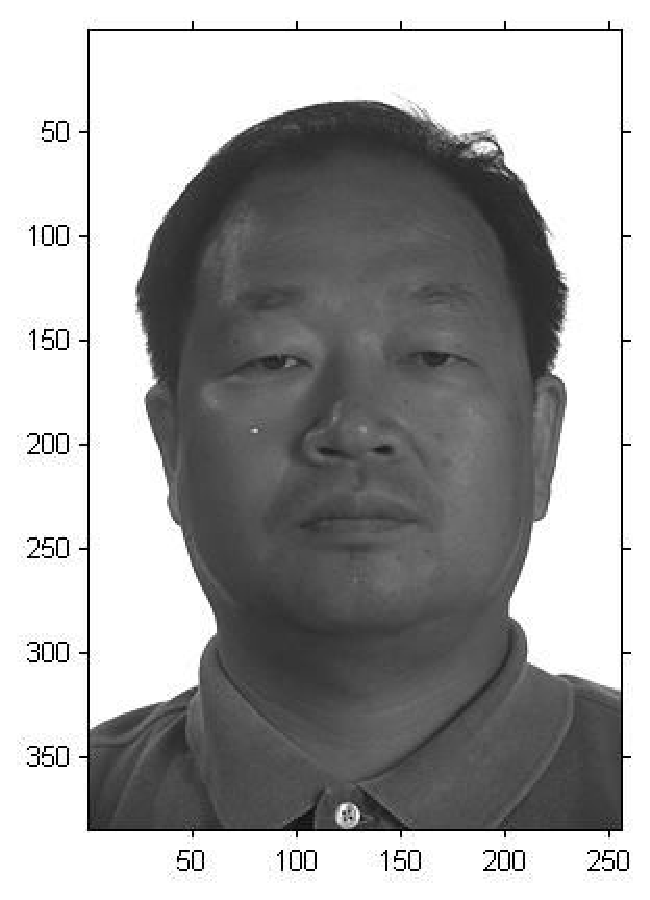
\includegraphics[width=3.3cm,height=2.7cm]{back5} &  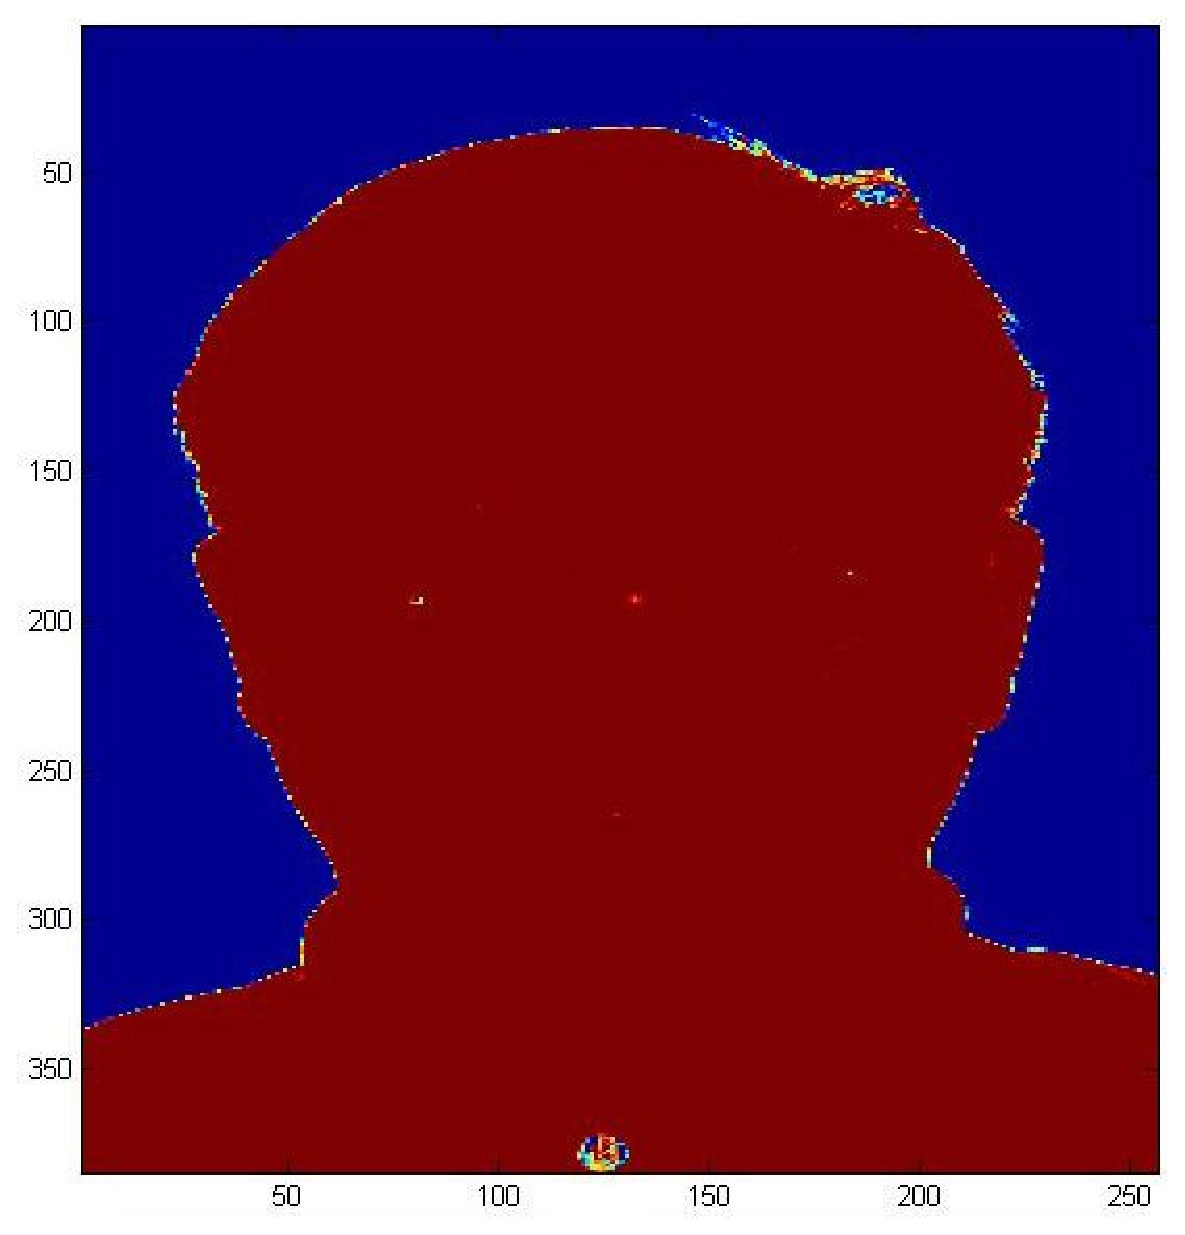
\includegraphics[width=3.3cm,height=2.7cm]{back2} \\
    \includegraphics[width=3.3cm,height=2.7cm]{back4} &  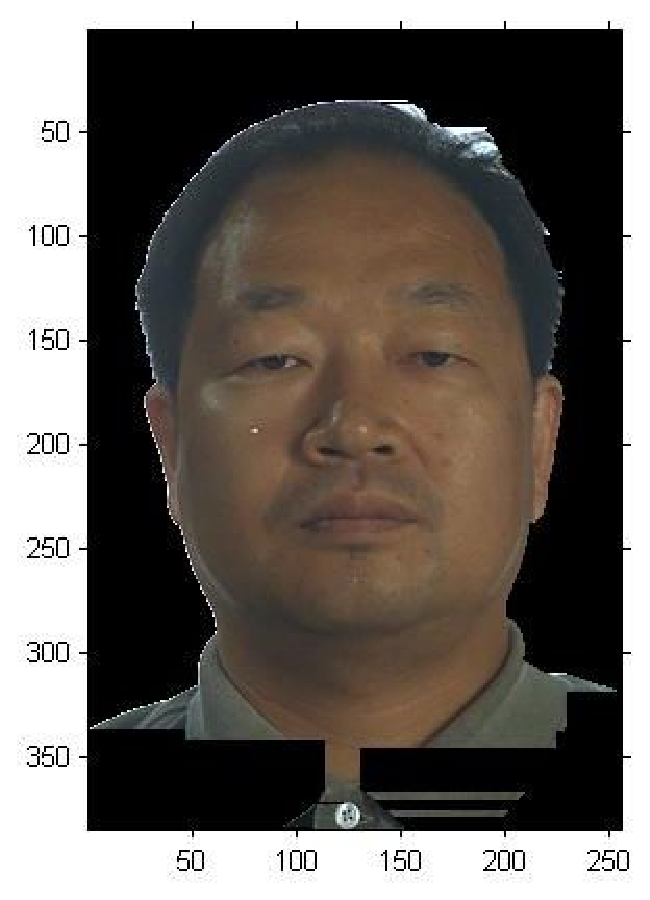
\includegraphics[width=3.3cm,height=2.7cm]{back6} \\
     \end{tabular}
Fig-2:- Figure depicting the facial images after background removal using DCT and edge detections
 \end{center}
 \end{table}

 \textbf{Algorithm}

\begin{itemize}
  \item The picture is applied with dct and idct, then this resultant is converted to integer of max 8 bits.
  \item The original image is subtracted from the reconstructed image after idct, and it is halved. In other words negative average of the idct and original image is taken
  \item The other method is to obtain the edges using sobel, then it is scanned and the required portion is extracted.
\end{itemize}

\subsection{Illuminations variations}
\hspace{1cm} the illuminations of the picture is of a greater concern as it is the one which models the image correlation. There are several techniques to overcome the illuminations like applying the log, dct, dwt, histogram based, white component based etc,\cite{two} . Here we have shown the left part before application of gamma equaliser and right side is the after gamma application in figure 3. and also histogram equalisation is shown in figure 4.
\begin{table}[htbp]
  \begin{center}
  \begin{tabular}{cc}
    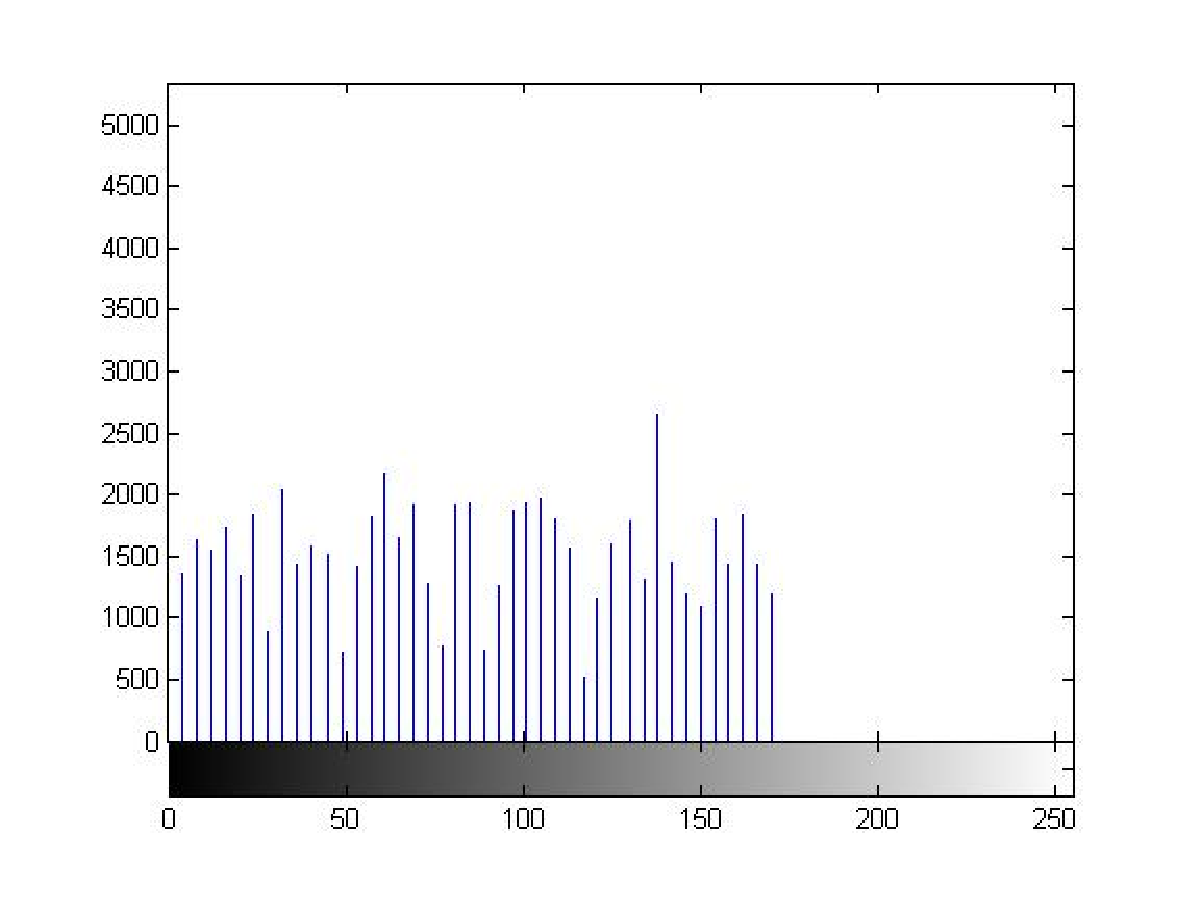
\includegraphics[width=3.3cm,height=2.7cm]{illu2} &  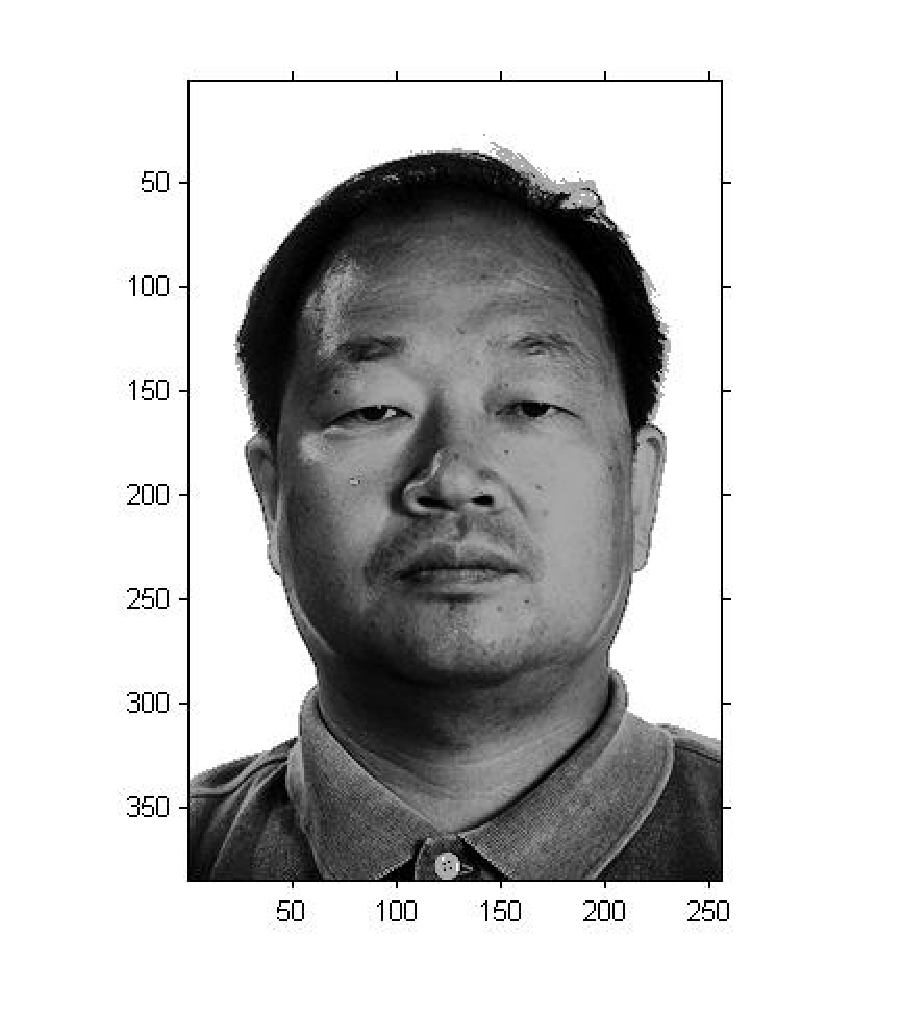
\includegraphics[width=3.9cm,height=2.7cm]{illu1} \\
     \end{tabular}
Fig-3:- Figure depicting the histogram technique after histogram equalisation
 \end{center}
 \end{table}
\begin{table}[htbp]
  \begin{center}
  \begin{tabular}{cc}
  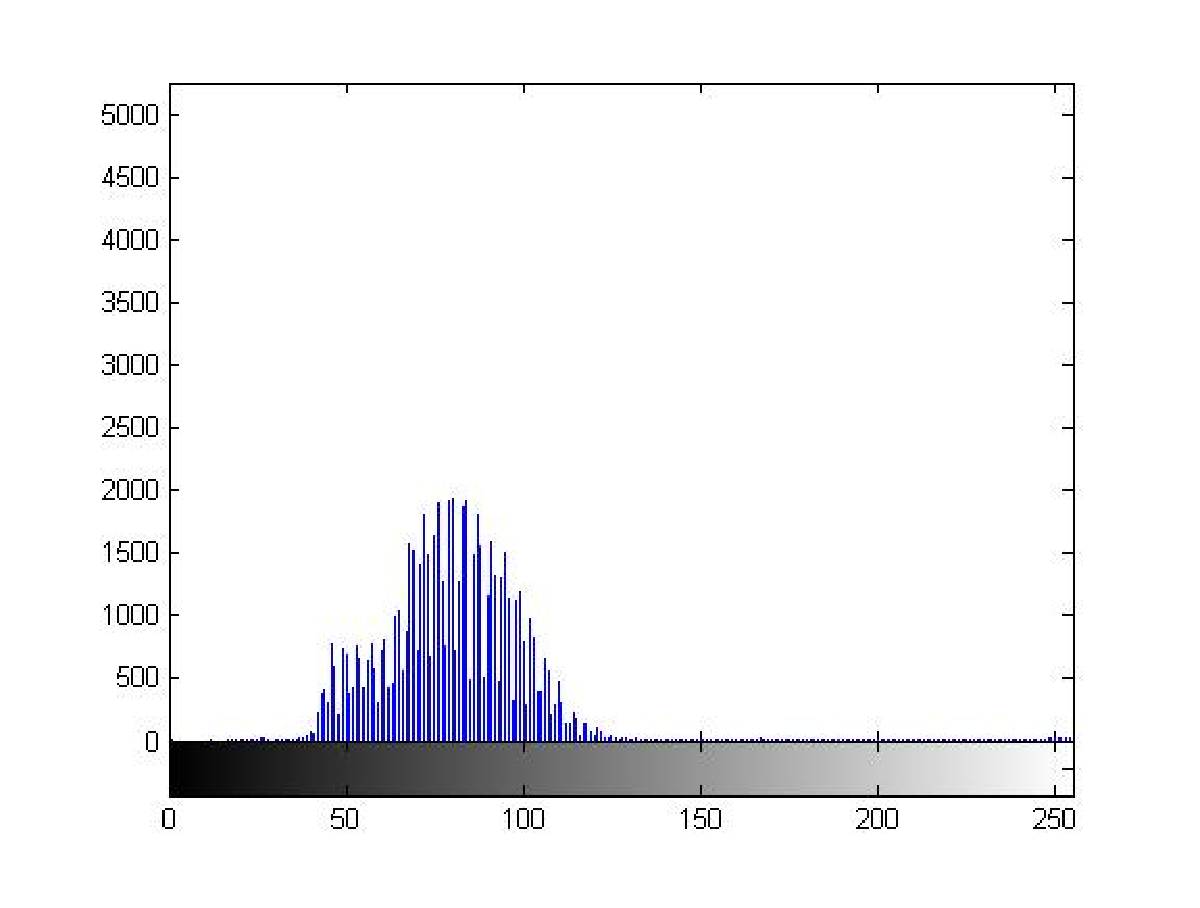
\includegraphics[width=3.3cm,height=2.7cm]{illu6} &  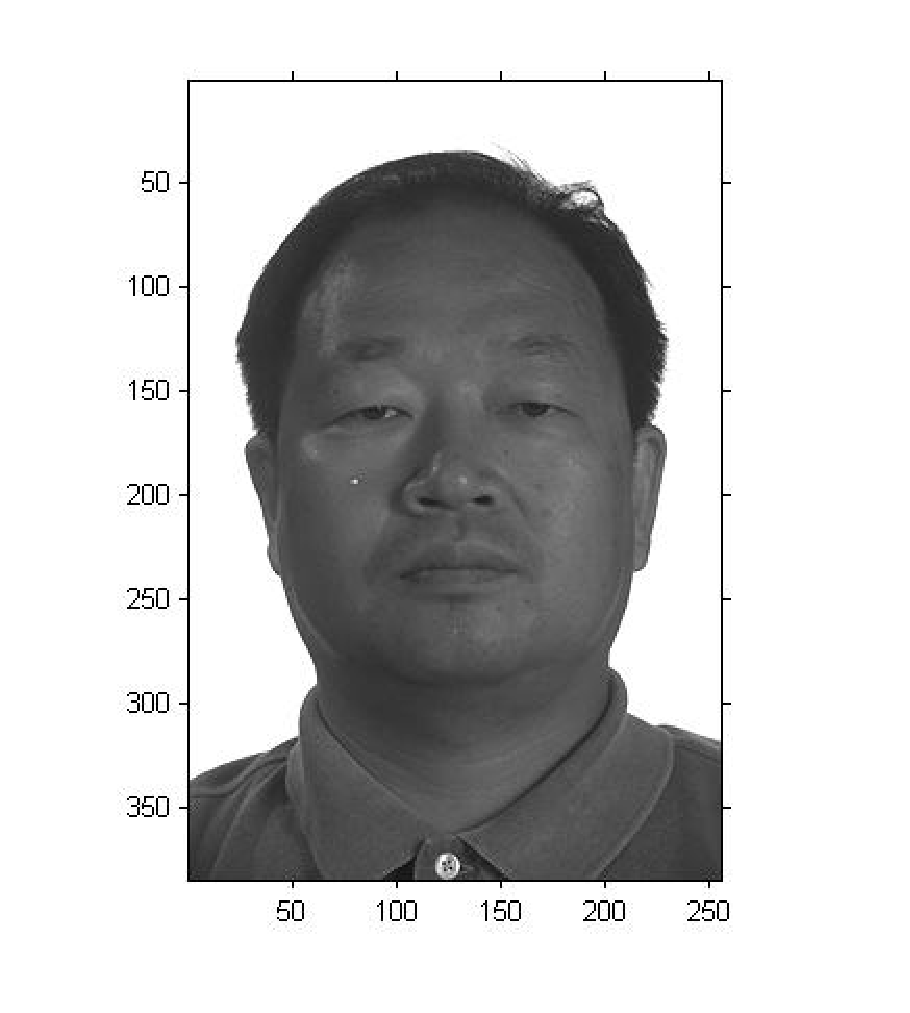
\includegraphics[width=3.9cm,height=2.7cm]{illu5} \\
    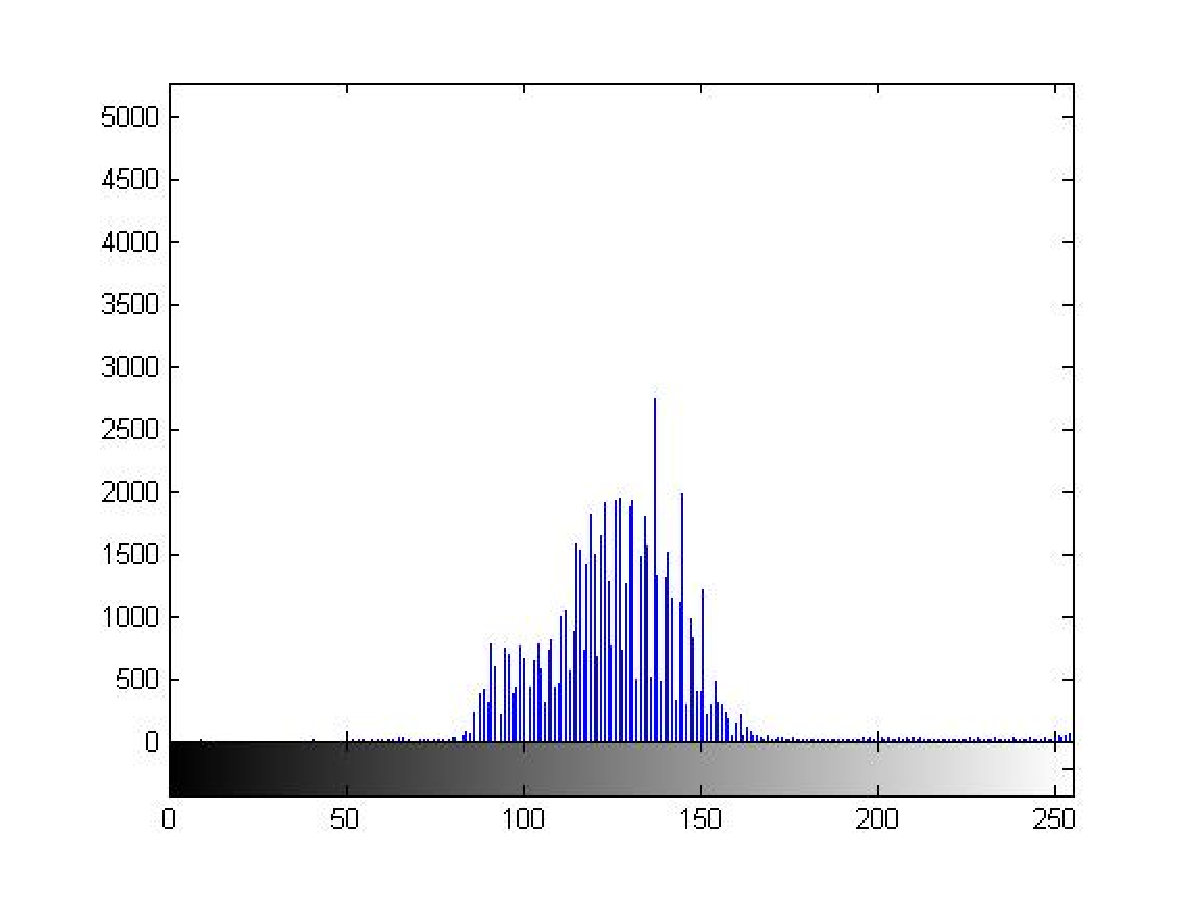
\includegraphics[width=3.3cm,height=2.7cm]{illu4} &  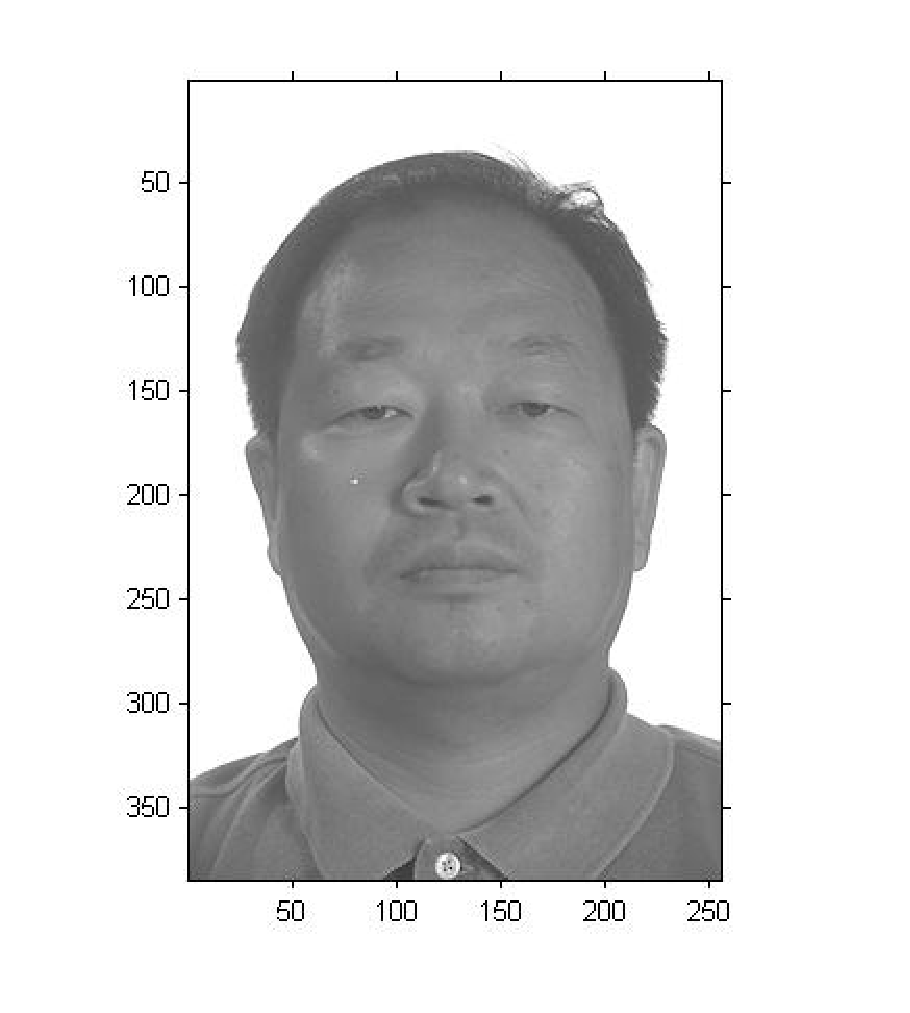
\includegraphics[width=3.9cm,height=2.7cm]{illu3} \\
     \end{tabular}
Fig-4:- Figure depicting the facial images after gamma application
 \end{center}
 \end{table}
\subsection{Template matching}
Here the eye part of the face is being detected using the pre-defined template.\\ $ $\\
\textbf{Algorithm}
\begin{itemize}
\item An eye template of predefined size is taken.
\item The normalized 2-D auto-correlation of eye template is found out.
\item the normalized 2-D cross-correlation of eye template with
various overlapping regions of the face image is calculated
\item The mean squared error  (MSE) of auto correlation and
cross-correlation of different regions are found out. The minimum
MSE is found out and stored.
\item the region of the face corresponding to minimum MSE
represents eye region
\end{itemize}
 \begin{center}
 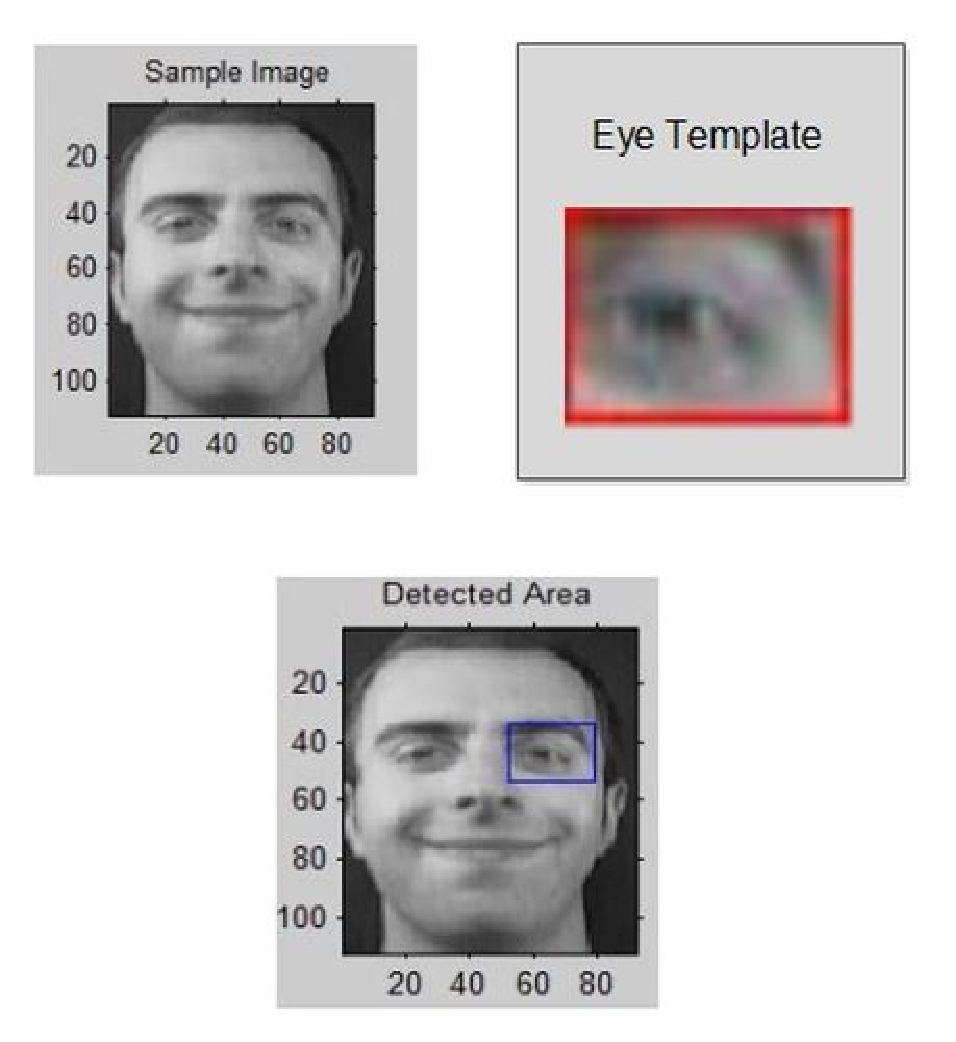
\includegraphics[width=6.6cm,height=5cm]{TempMatching}\\
  Fig-5:Figure Showing the working of template matching\\
 \end{center}

Here the correlation coefficient calculation is implemented not with built-in function corr or corr2 but with conv2 so that the template matching speed has been accelerated and run-time has reduced to a reasonable value.Because the
function corr is relatively slow for template matching purpose and it is also required extra considerations on controlling the boundary and selecting region of interest on the frame image.

\subsection{Skin color segmentation}
This method is used to detect the only the skin part based on the segmentation\cite{four}.\\ $ $\\
\textbf{Algorithm}
\begin{itemize}
\item To compensate for the lighting effects colour balancing is done first.
\item Then the thresholding is done in Ycgcr and HSV Colour space to get the skin part.
\item Now the holes in the faces are to be filled.
\item  Eliminating Pixels Below a Threshold.
\item Putting Bounding Boxes Around Detected Faces.
\end{itemize}

\begin{center}
 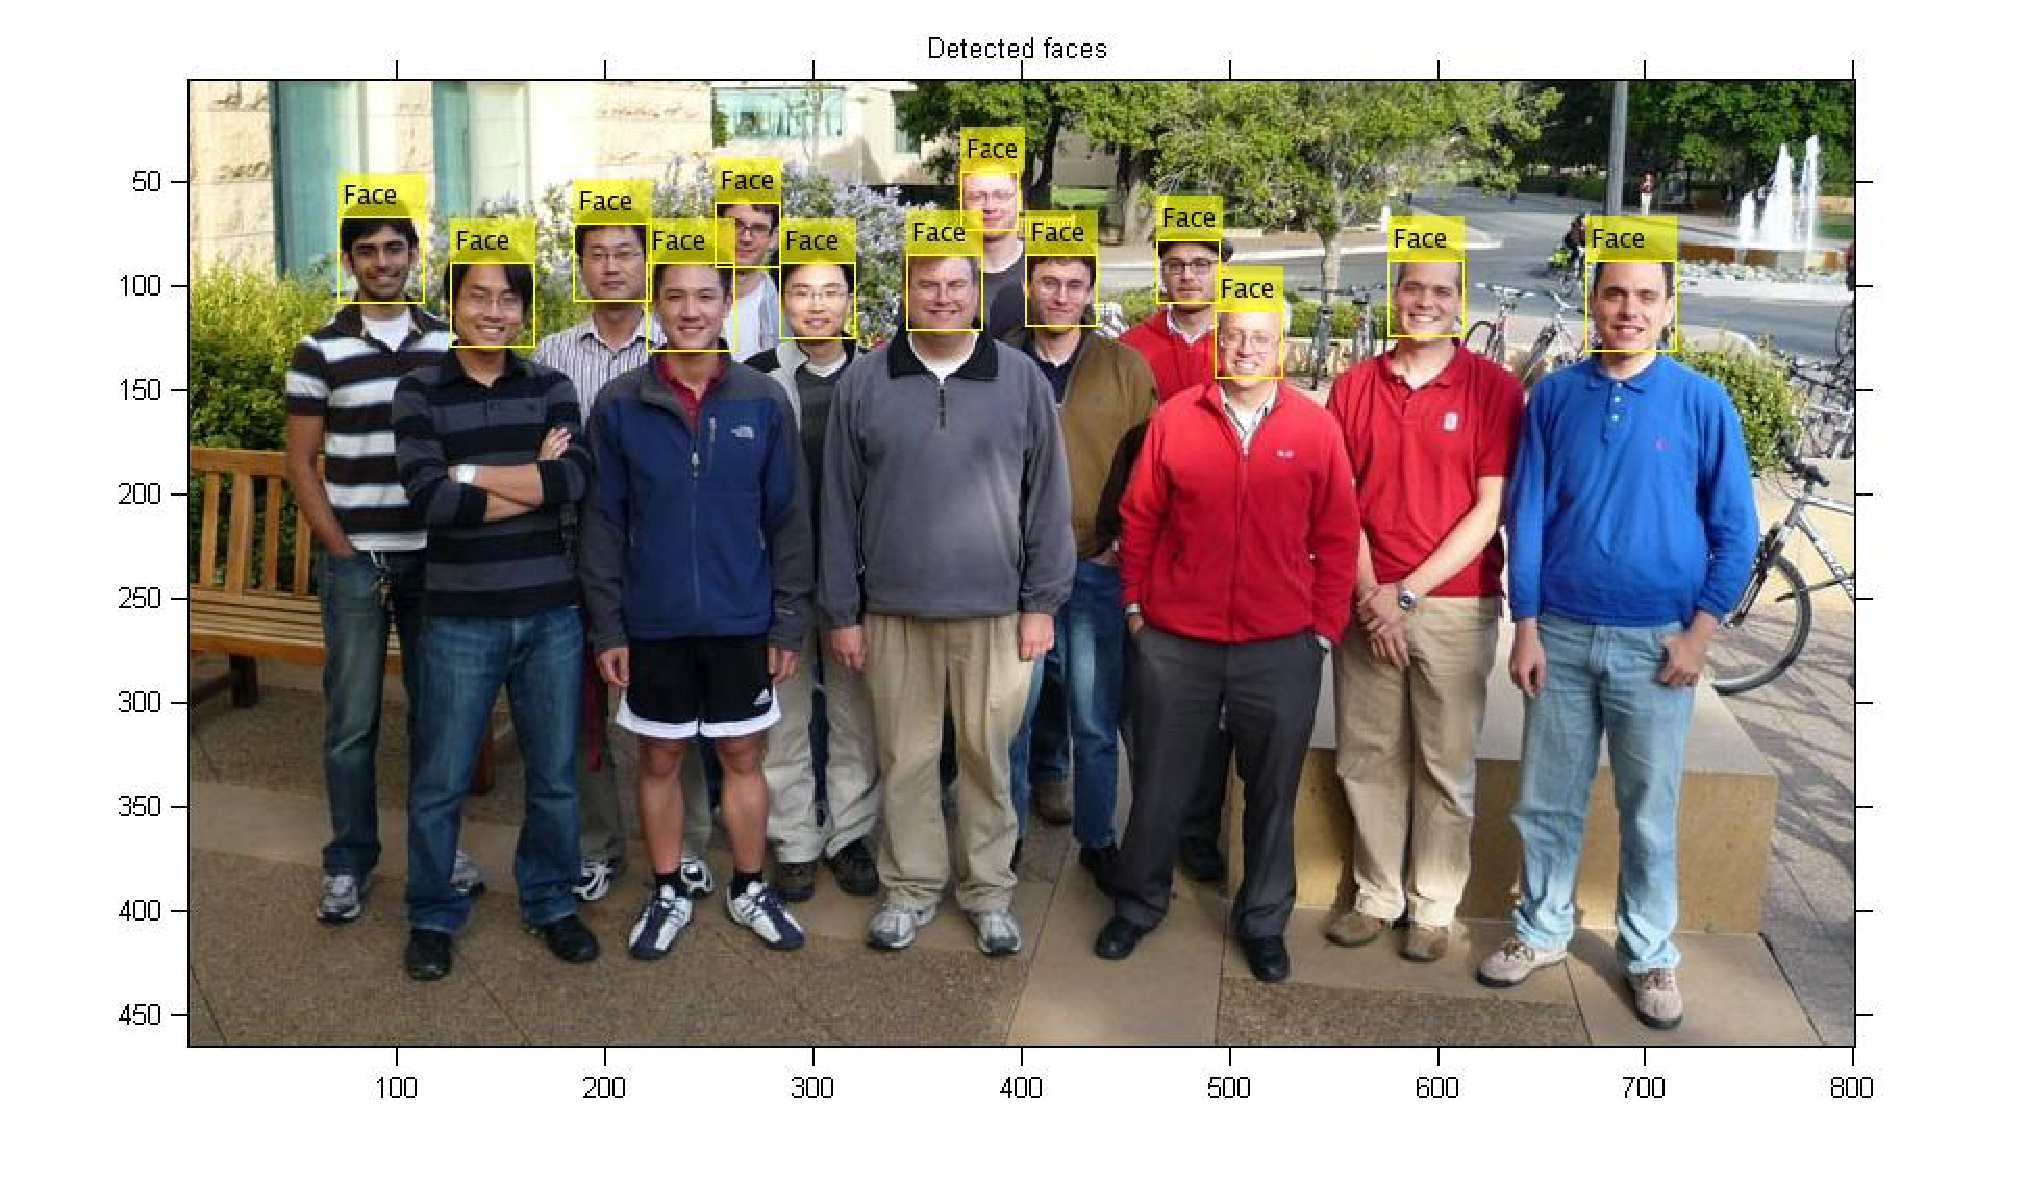
\includegraphics[width=6.6cm,height=5cm]{det_pic}\\
  Fig-6:Figure Showing the detected faces in a group\\
 \end{center}

\subsection{2D Normalized Cross Correlation}
\hspace{1cm} The correlation of any image is defined as the inverse of the variance between the pixels. The cross correlation is just the correlation but here the image is compared with other images. 2D normalisation is important as such the entropy is equally distributed. \\
\hspace{1cm} The Figure 7 shows the template eye is perfectly matched and is marked in the figure
\begin{table}[htbp]
  \begin{center}
  \begin{tabular}{cc}
    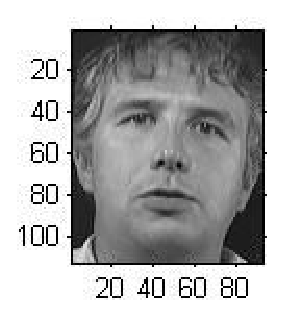
\includegraphics[width=3.3cm,height=2.7cm]{cross1} &  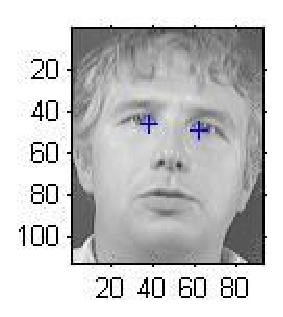
\includegraphics[width=3.9cm,height=2.7cm]{cross2} \\
    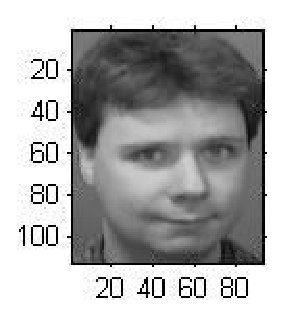
\includegraphics[width=3.3cm,height=2.7cm]{cross3} &  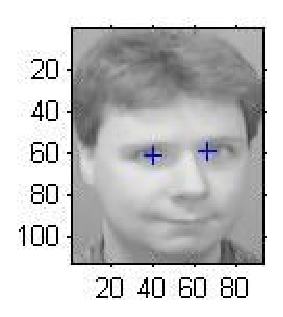
\includegraphics[width=3.9cm,height=2.7cm]{cross4} \\
     \end{tabular}
Fig-7:- Figure depicting the eye template correlated with different images
 \end{center}
 \end{table}

 \subsection{Geometric Normalisation}
 \hspace{1cm} The faces in the images are aligned differently due to reason of pose variance. The eye, nose, mouth, etc., are the important features which have to be aligned properly in every image so as to get a maximum class separation. This method of aligning the faces so as to get the geometrically equivalent figures is known as geometric normalisation\cite{five}.

\begin{table}[htbp]
  \begin{center}
  \begin{tabular}{cc}
    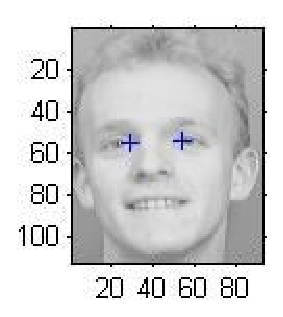
\includegraphics[width=3.3cm,height=2.7cm]{geo1} &  
\includegraphics[width=3.9cm,height=2.7cm]{geo2} \\
     \end{tabular}
Fig-8:- Figure depicting the eye template correlated face angle tilted geometric normalisation.
 \end{center}
 \end{table}

 \textbf{Algorithm}
\begin{itemize}
  \item Firstly the eyes in the image are located using dct, cross correlation, template matching etc.
  \item The co-ordinates of eyes are marked and a line is drawn to join these points.
  \item Finally the face(image) is tilted to have the joint line in parallel to the horizontal axis.
\end{itemize}

\section{Conclusion}
\begin{itemize}
  \item The image is pre-processed using the above techniques so as to have the proper class separation.
  \item The image is trained so as to get the proper alignment and this will help in removing pose variations
  \item Main aim of doing pre-processing is to remove the redundancy and other unwanted objects and to have exactly the face with the required important features.
\end{itemize}



\section*{References}

\begin{thebibliography}{9}

\bibitem{One}
Fergus, Rob, Pietro Perona, and Andrew Zisserman. "Object class recognition by unsupervised scale-invariant learning." Computer Vision and Pattern Recognition, 2003. Proceedings. 2003 IEEE Computer Society Conference on. Vol. 2. IEEE, 2003.

\bibitem{two}
Phong, Bui Tuong. "Illumination for computer generated pictures." Communications of the ACM 18.6 (1975): 311-317.

\bibitem{three}
Gordon, G., et al. "Background estimation and removal based on range and color." Computer Vision and Pattern Recognition, 1999. IEEE Computer Society Conference on.. Vol. 2. IEEE, 1999.

\bibitem{four} Wang, Baozhu, Xiuying Chang, and Cuixiang Liu. "Skin Detection and Segmentation of Human Face in Color Images."

\bibitem{five}Starovoitov, V. V., D. I. Samal, and D. V. Briliuk. "Three approaches for face recognition." The 6-th International Conference on Pattern Recognition and Image Analysis, Velikiy Novgorod, Russia. 2002.

\end{thebibliography}
\end{document}
